%-- einleitung

\section{Einführung}
In der Informatik und Mathematik wünscht man sich für eine konkrete Problemstellung eine exakte Lösung. Allerdings gibt es Probleme, für die es bis heute keine deterministischen Algorithmen gibt, die diese Aufgaben in polynomieller Zeit lösen. 
Ein Grund dafür kann zum Beispiel sein, dass es für die Lösung eines Problems zu viele Kombinationsmöglichkeiten gibt, die zu überprüfen sind, bis ein exaktes Ergebnis angegeben werden kann. Ein solcher Algorithmus, der in der Klasse der NP-schweren Probleme liegt, ist das Travelling Salesman Problem (TSP).
Diese Tatsache ändert allerdings nichts daran, dass auch für solche Probleme Lösungen gefunden werden müssen. Aus diesem Grund wird die Lösung approximiert. Es wird also ein Ergebnis gesucht, das möglichst nah an der exakten Lösung liegt. 
Die Genetischen Algorithmen bieten die Möglichkeit über die Nachahmung von evolutionären Vorgängen eine eben solche Approximierung durchzuführen.
Dabei wird aus einer Menge an anfänglich schlechten Lösungen durch Rekombination, Mutation und Selektion das Ergebnis schrittweise verbessert. In der folgenden Ausarbeitung wird beschrieben wie ein eigens implementierter Genetischer Algorithmus das TSP löst.

\subsection{Ziele}
Das Ziel dieses Projektes ist es zum einen ein System zu entwickeln, das die Möglichkeiten von Genetischen Algorithmen am Beispiel des Travelling-Salesman-Problem demonstriert.
Zum anderen soll untersucht werden welche Stellschrauben der Genetischen Algorithmen die Resultate inwieweit positiv oder negativ beeinflussen.

\subsection{Genetische Algorithmen}
Bei Genetischen Algorithmen \cite[S. 130-132]{tsp} handelt es sich um eine Klasse von Optimierungs-Algorithmen, die sich an den evolutionären Vorgängen in der Natur orientieren. Diese Algorithmen approximieren lediglich Probleme und finden so nur durch Zufall eine optimale Lösung.
Die Genetischen Algorithmen wurden im Fachvortrag zu den Evolutionsstrategien schon näher erläutert und werden im Folgenden lediglich zusammengefasst.\\
In Abbildung \ref{fig:genetic_algorithm} ist eine Übersicht der Abläufe innerhalb der Genetischen Algorithmen zu sehen. Individuen werden als Spielkarten dargestellt und Populationen als Kartenstapel. Individuen beinhalten die zu verändernden Informationen, die sogenannten Chromosome. Die Individuen sind zu Beginn zufällig initialisiert.
Für jedes Individuum lässt sich eine Bewertung und eine Fitness berechnen. Die Bewertung gibt eine Aussage darüber, wie nah ein Individuum an einer optimalen Lösung liegt.
Die Fitness entspricht der Wahrscheinlichkeit, dass ein Individuum zur Fortpflanzung ausgewählt wird und wird aus der Bewertung berechnet. Es ist dabei auch möglich, dass die Bewertungs- und Fitnessfunktion identisch oder sehr ähnlich sind.
Der erste wichtige Ablauf innerhalb der Genetischen Algorithmen ist die Wahl geeigneter Elternindividuen. Diese Auswahl wird Hochzeit genannt. Je höher die Fitness des Individuums, desto höher ist auch die Wahrscheinlichkeit, dass es als Elternindividuum ausgewählt wird.
Typischerweise werden aus zwei Elternindividuen zwei Nachkommen gebildet. Dieser Vorgang wird Crossover genannt und schließt eine Rekombination der Elternchromosome mit ein. Anschließend wird, mit einer vorgegeben Ausführungsrate, eine Mutation durchgeführt. In der Abbildung ist dies als Übergang von Kind C zu C` zu sehen. Das Kind D bleibt unverändert.
Hochzeit, Crossover und Mutation werden so lange durchgeführt, bis die Endpopulation so groß ist wie die Startpopulation. Anschließend wird aus diesen Populationen eine neue Startpopulation gebildet. Dazu können zum Beispiel die fittesten Individuen der beiden Populationen ausgewählt werden.
Die Selektion schließt einen Generationsschritt ab. Dies wird so lange wiederholt, bis die Startpopulation die gewünschte Qualität hat oder eine vorgegebene Anzahl an Generationsschritten durchgeführt wurde.
Anwendungsmöglichkeiten für die Genetischen Algorithmen finden sich unter anderem in der Ökonomie, Mustererkennung und im maschinellen Lernen \cite[S. 185-186]{schoeneburg}.

\begin{figure}[H]
\centering
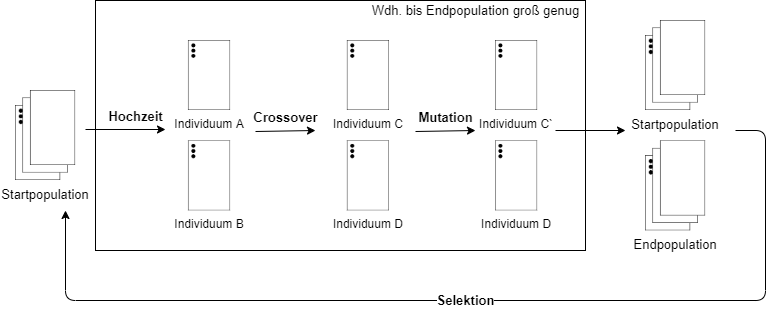
\includegraphics[width=1\textwidth]{img/Vortrag/Genetic_Algorithm.png}
\caption{Überblick über die Abläufe der Genetischen Algorithmen}
\label{fig:genetic_algorithm}
\end{figure}

\subsection{Travelling Salesman Problem}
Das Travelling Salesman Problem \cite[S. 132-133]{tsp} (TSP), oder auch Problem des Handlungsreisenden genannt, beschreibt ein Optimierungsproblem, bei dem ein Handlungsreisender eine Menge an Städten nacheinander besucht. Die Vorgabe ist zum einen, dass jede Stadt außer der Startstadt genau einmal besucht werden darf und zum anderen soll die zurückgelegte Distanz minimal sein. Dabei ist zu beachten, dass zwischen allen Städten die Distanzen bekannt sein müssen.
Eine beispielhafte Lösung des TSP ist in Abbildung \ref{fig:TSP} zu sehen. Dieses unkompliziert wirkende Problem ist allerdings nicht einfach zu lösen, weil es bei einer Menge an Städten eine große Anzahl an verschiedenen Kombinationsmöglichkeiten gibt. Bei 20 Städten gibt es schon $20!$ Möglichkeiten, was ungefähr $10^(18)$ Möglichkeiten entspricht die Städte anzuordnen. Dies schließt eine Lösung nach dem Ansatz der rohen Gewalt bereits aus. Darüber hinaus befindet sich das TSP in der Kategorie der NP-schweren Probleme. Es gibt also keinen bekannten Algorithmus, der das Problem in deterministisch polynomieller Zeit löst. Aus diesem Grund ist die Untersuchung des TSP mit den Genetischen Algorithmen besonders interessant.

\begin{figure}[H]
\centering
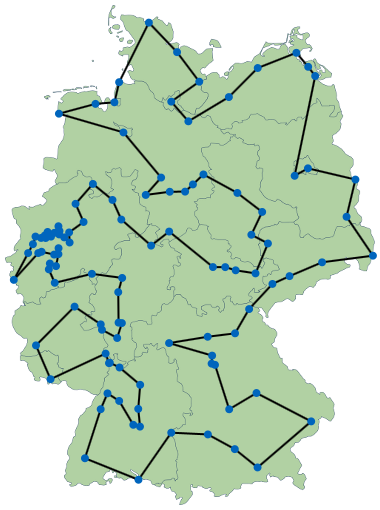
\includegraphics[width=0.4\textwidth]{img/Vortrag/tsp.png}
\caption{Travelling Salesman Problem}
\label{fig:TSP}
\end{figure}

\subsection{Struktur der Arbeit}
Die Ausarbeitung beginnt mit einer Übersicht über die konzeptionelle Planung, die dem eigentlichen Projekt vorangegangen ist. Dazu wurde eine Anforderungsanalyse und eine Systemmodellierung durchgeführt. Anschließend folgt die Umsetzung des gefundenen Konzepts. Dabei werden grundlegende Entscheidungen, wie die Wahl von Programmiersprachen und Bibliotheken, erläutert. Darüber hinaus wird in diesem Abschnitt auf einzelne Projektabschnitte mit Codebeispielen eingegangen. Die Realisierung wird danach mit einigen Experimenten getestet und dabei die Genetischen Algorithmen im Allgemeinen untersucht. Die Ausarbeitung schließt mit einem Fazit der Ergebnisse und einem Ausblick ab.


%--